\documentclass[usenames,dvipsnames]{beamer}
\usepackage{xcolor}
\usepackage{tcolorbox}
\usepackage{graphicx}
\usepackage{amsmath}
\usepackage{subcaption}
\usepackage{makecell}
\usepackage[labelformat=empty]{caption}
\usepackage{color, colortbl}
\usepackage{booktabs}
\usepackage{pdfpages}
\usepackage{multirow}
\usepackage{comment}
\usepackage{hyperref}
\hypersetup{
    colorlinks=true,
    linkcolor=blue,
    filecolor=magenta,      
    urlcolor=cyan,
}

\newcommand*{\mathcolor}{}
\def\mathcolor#1#{\mathcoloraux{#1}}
\newcommand*{\mathcoloraux}[3]{%
	\protect\leavevmode
	\begingroup
	\color#1{#2}#3%
	\endgroup
}

\usepackage{tikz}

\usetikzlibrary{shapes.geometric, arrows}
\tikzstyle{startstop} = [rectangle, rounded corners, minimum width=3cm, minimum height=1cm,text centered, draw=black, fill=brown!30]

\tikzstyle{io} = [trapezium, trapezium left angle=70, trapezium right angle=110, minimum width=3cm, minimum height=1cm, text centered, draw=black, fill=blue!30]

\def\checkmark{\tikz\fill[scale=0.4](0,.35) -- (.25,0) -- (1,.7) -- (.25,.15) -- cycle;} 

\tikzstyle{arrow} = [thick,->,>=stealth]


\newcommand{\DoTikzmark}[1]{%
	\tikz[remember picture] \coordinate[shift={(0,.7ex)}](#1);%
}

\newcommand{\colrow}[3][]{%
	\tikz[overlay,remember picture, line width=10pt]
	\draw[shorten >=-.1em, shorten <=-.1em, #1] (#2)--(#3);
}


\newcolumntype{g}{>{\columncolor{Lavender}}c}
\newcolumntype{t}{>{\columncolor{Tan}}c}

%\beamerdefaultoverlayspecification{<+->}
\newcommand{\data}{\mathcal{D}}

\DeclareMathOperator*{\argmin}{arg\,min}

\newcommand\Item[1][]{%
	\ifx\relax#1\relax  \item \else \item[#1] \fi
	\abovedisplayskip=0pt\abovedisplayshortskip=0pt~\vspace*{-\baselineskip}}
	


\usetheme{metropolis}           % Use metropolis theme


\title{K-Nearest Neighbors}
\date{\today}
\author{Nipun Batra}
\institute{IIT Gandhinagar}
\begin{document}
  \maketitle

{
	\setbeamercolor{background canvas}{bg=}
	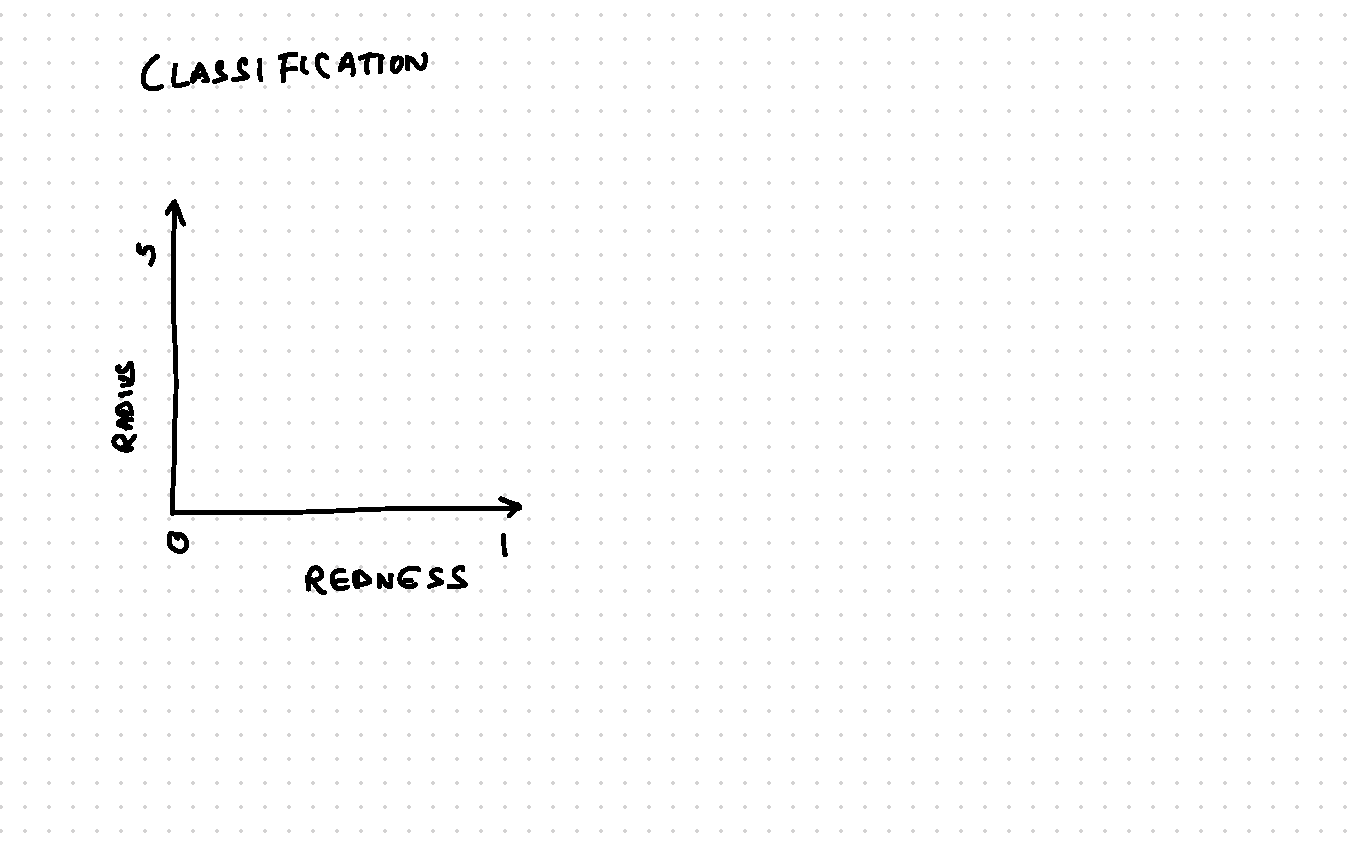
\includepdf[page=-]{knn/knn-intuition.pdf}
}

{
	\setbeamercolor{background canvas}{bg=}
	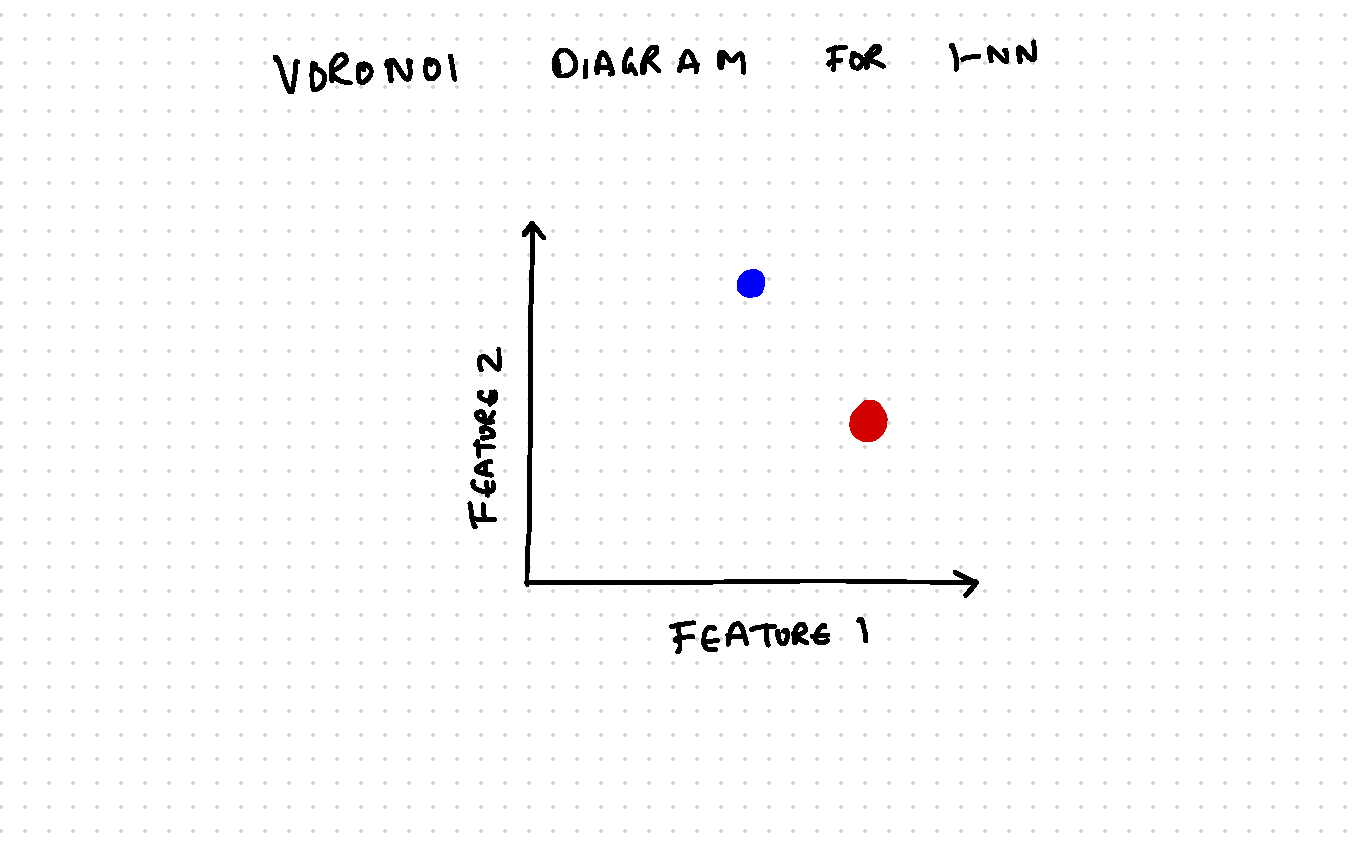
\includepdf[pages=1-20]{knn/1nn.pdf}
}


\begin{frame}{Parametric vs Non-Parametric Models}
\begin{table}[]
\begin{tabular}{|l|p{3.5cm}|p{3.5cm}|}
\hline
            & Parametric                                               & Non-Parametric                                                   \\ \hline
Parameter   & Number of parameters is fixed w.r.t dataset size         & Number of parameters grows w.r.t. to an increase in dataset size \\ \hline
Speed       & Quicker (as the number of parameters are less)           & Longer (as number of parameters are less)                        \\ \hline
Assumptions & Strong Assumptions (like linearity in Linear Regression) & Very few (sometimes no) assumptions                              \\ \hline
Examples    & Linear Regression                                        & KNN, Decision Tree                     \\ \hline                         
\end{tabular}
\end{table}
\end{frame}

\begin{frame}{Lazy vs Eager Strategies}
	\begin{table}[]
		\begin{tabular}{|l|p{3.5cm}|p{3.5cm}|}
			\hline
			& Lazy                                     & Eager                                   \\
			\hline
			Train Time & $0$                                      & $\neq 0$                                \\
			\hline
			Test       & Long (due to comparison with train data) & Quick (as only ``parameters'' are involved) \\
			\hline
			Memory     & Store/Memorise entire data               & Store only learnt parameters            \\
			\hline
			Utility    & Useful for online settings               &                                         \\
			\hline
			Examples   & KNN                                      & Linear Regression, Decision Tree       \\ \hline
		\end{tabular}
	\end{table}
\end{frame}

\begin{frame}{Important Considerations}
\begin{itemize}
\item<1-> What are the \textbf{features} that will be considered for data similarity?
\item<2-> What is the \textbf{distance metric} that will be used to calculate data similarity?
\item<3-> What is the \textbf{aggregation function} that is going to be used?
\item<4-> What are the \textbf{number of neighbors} that you are going to take into consideration?
\item<5-> What is the \textbf{computational complexity} of the algorithm that you are implementing?
\end{itemize}
\end{frame}

\begin{frame}{Important Considerations: Distance Metric}
The Distance Metric acts as a \emph{measure of similarity} between the points.

{\centering
\only<2>{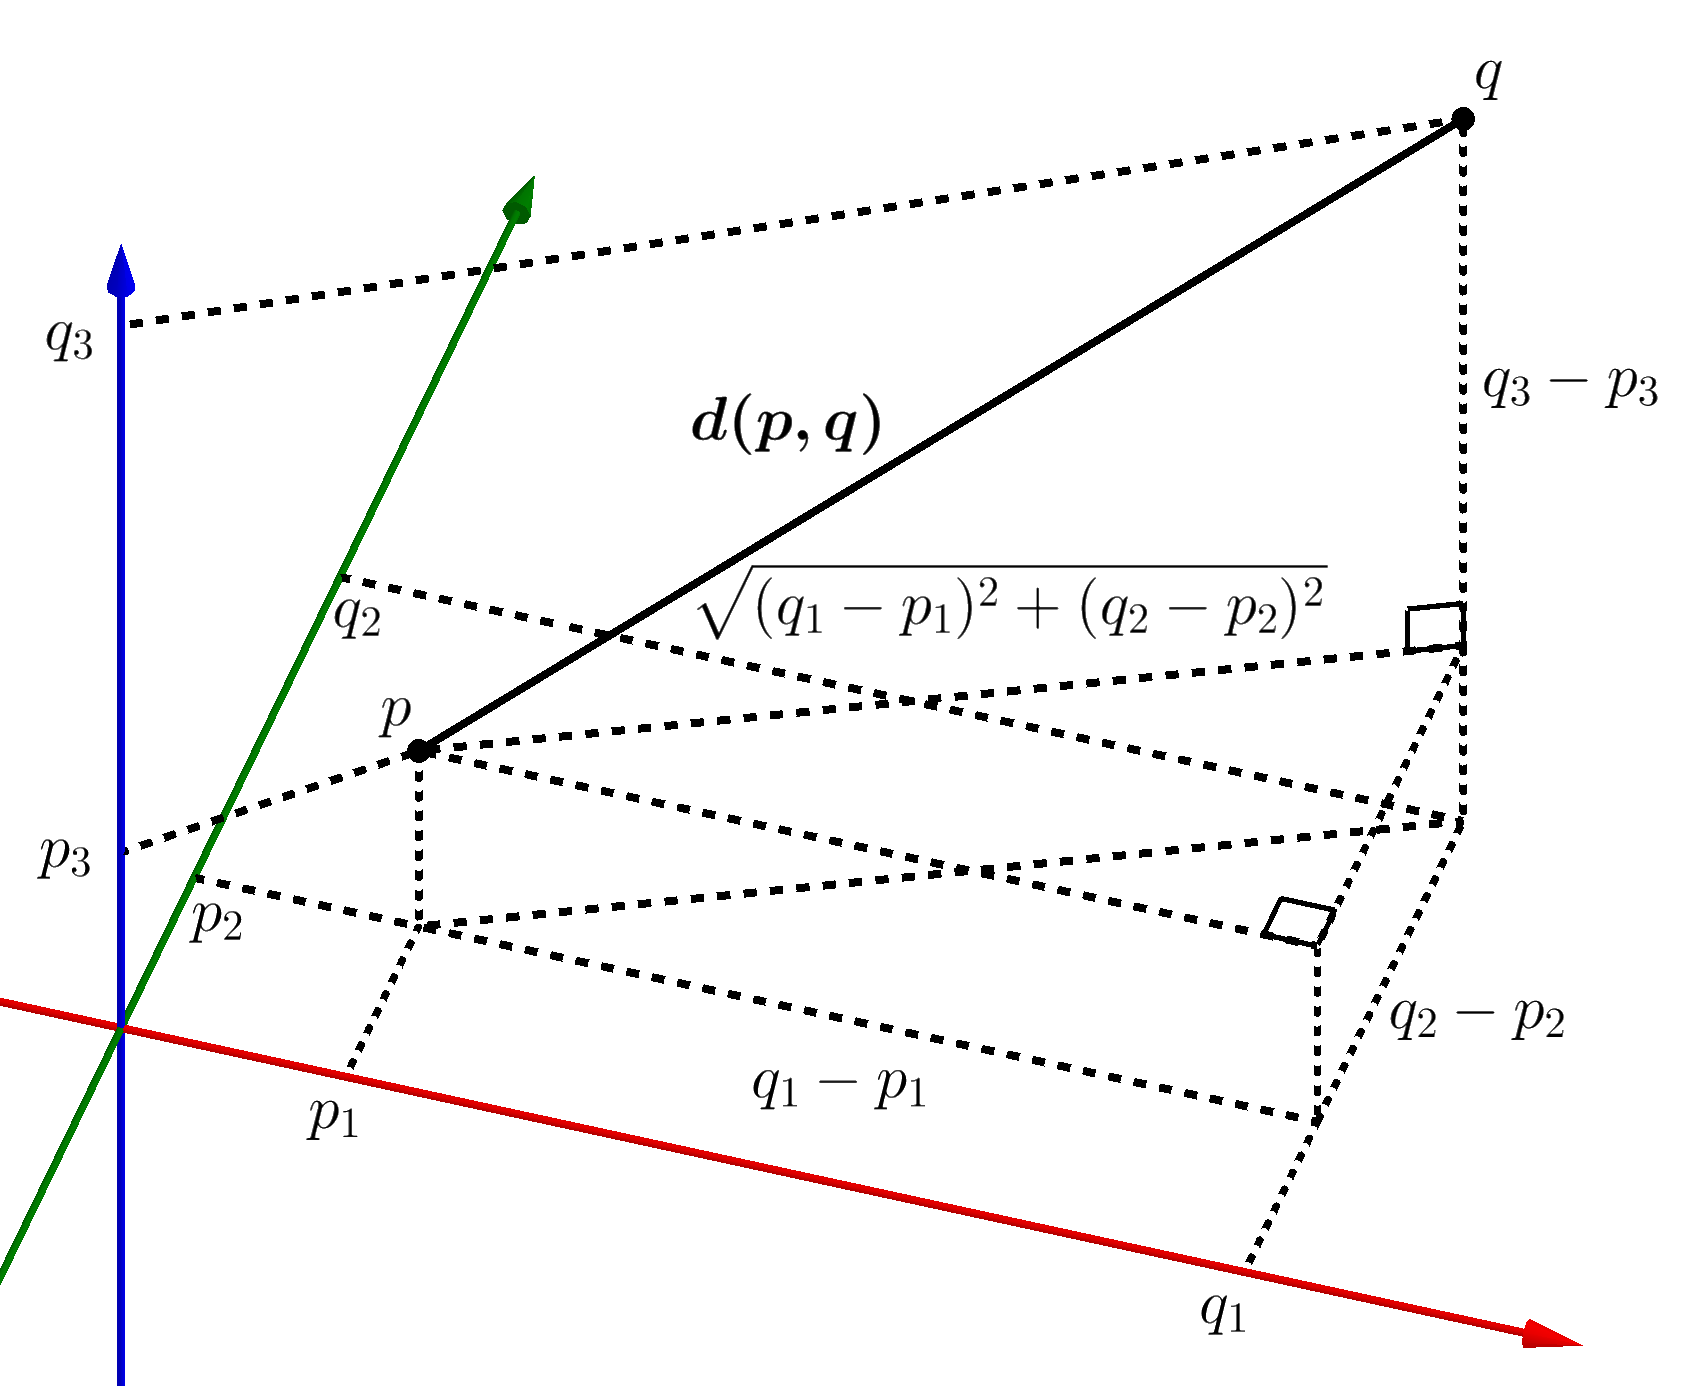
\includegraphics[height=0.6\textheight]{knn/knn_ed.png}
\captionof{figure}{Euclidean Distance}}
\only<3>{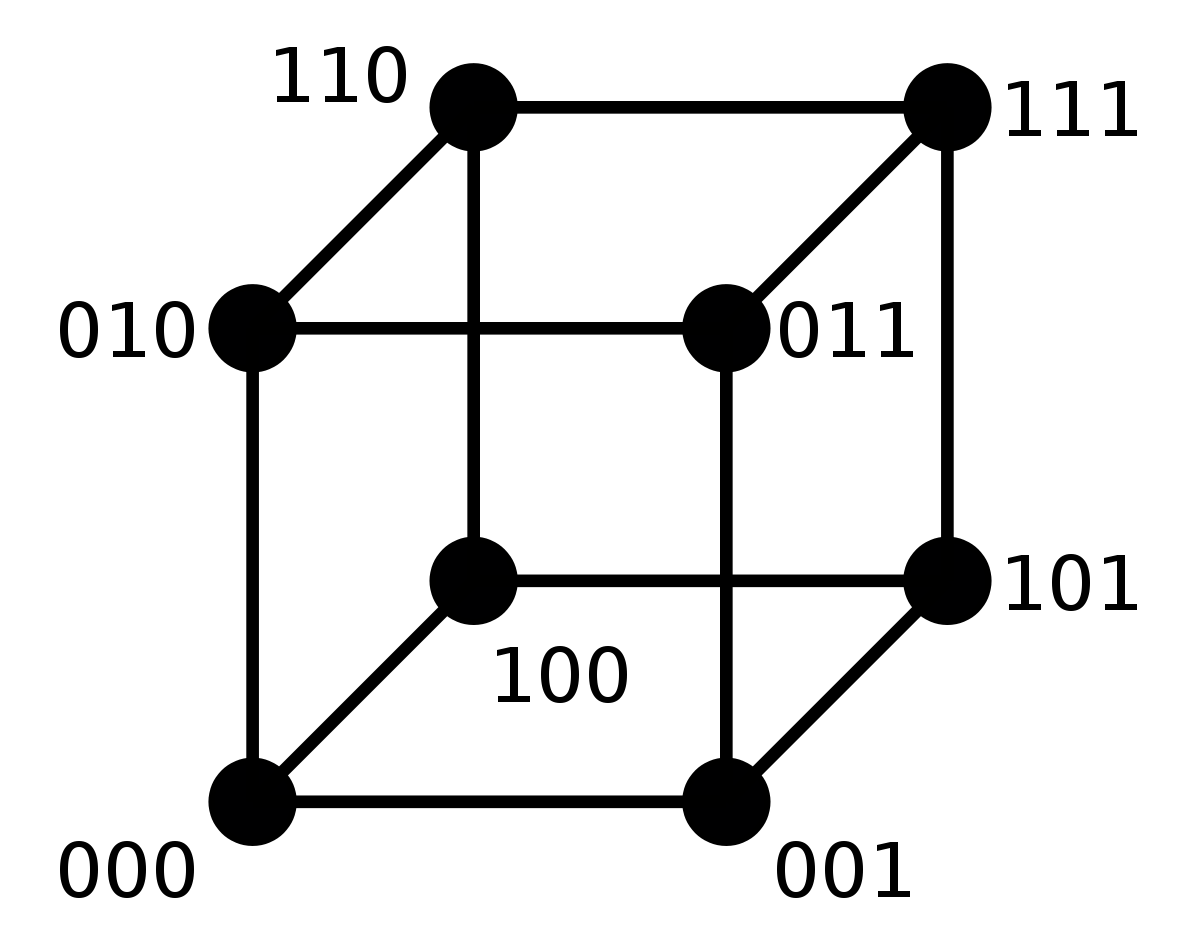
\includegraphics[height=0.6\textheight]{knn/knn_hd.png}
\captionof{figure}{Hamming Distance}}
\only<4>{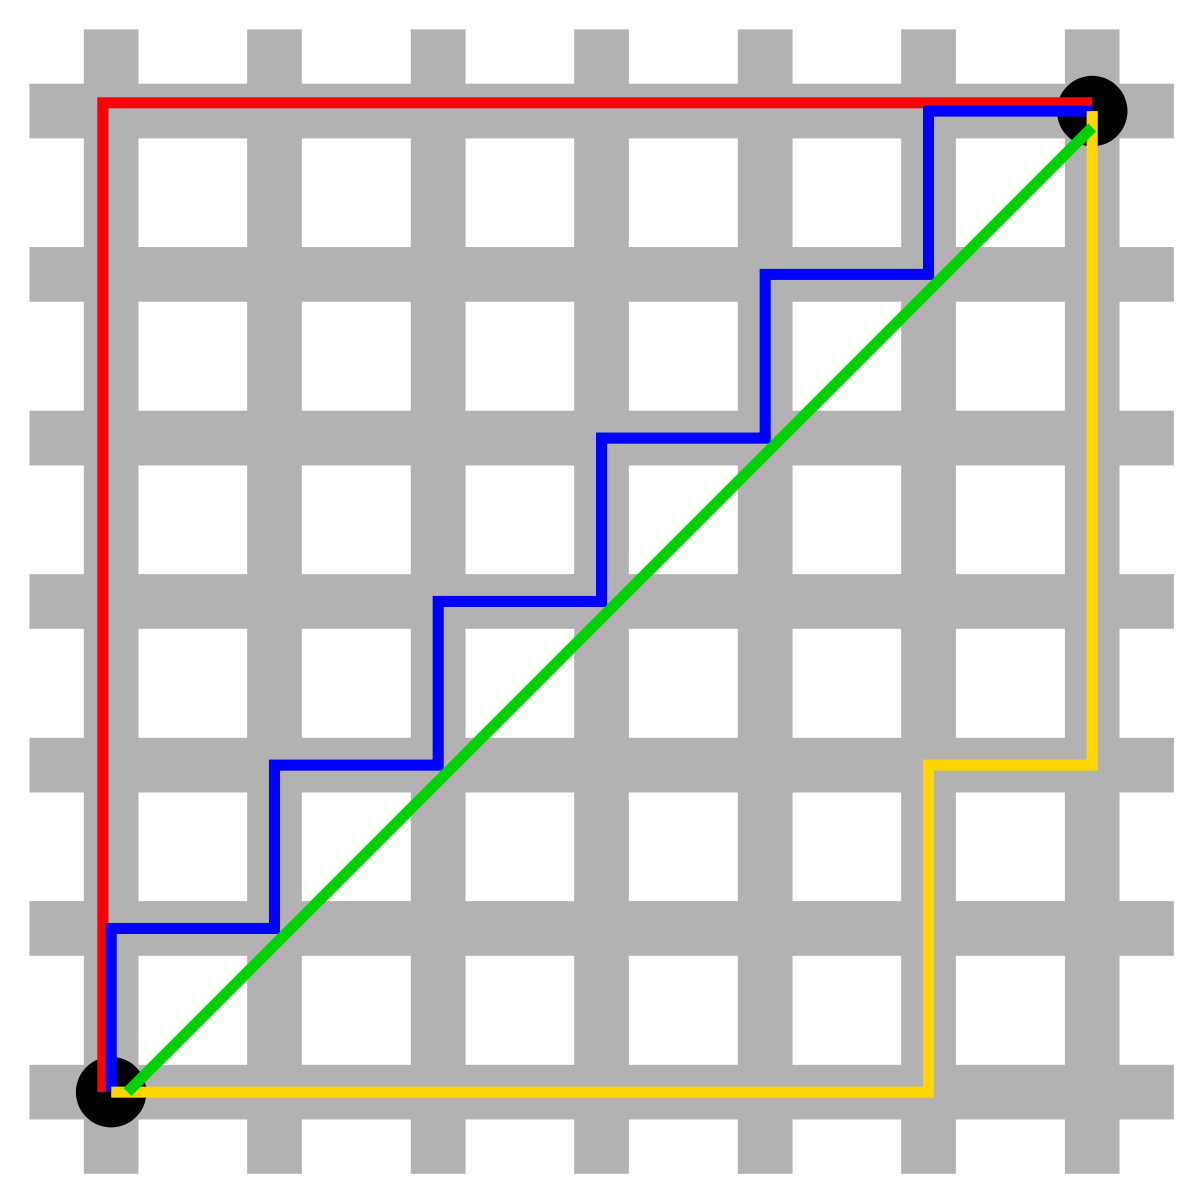
\includegraphics[height=0.6\textheight]{knn/knn_md.png}
\captionof{figure}{Manhattan Distance}}}

%\only<5>{
%Choose the best distance metric \textbf{based on the properties of the data}. 

%Euclidean is a good distance measure to use if the input variables are similar in type (e.g. all measured widths and heights). Manhattan distance is a good measure to use if the input variables are not similar in type (such as age, gender, height, etc.).

%\href{https://machinelearningmastery.com/k-nearest-neighbors-for-machine-learning/}{More Info}}
\end{frame}


\begin{comment}


\begin{frame}{Important Considerations: Distance Metric}
Variation of decision boundaries of a random data set
\begin{figure}
    \centering
    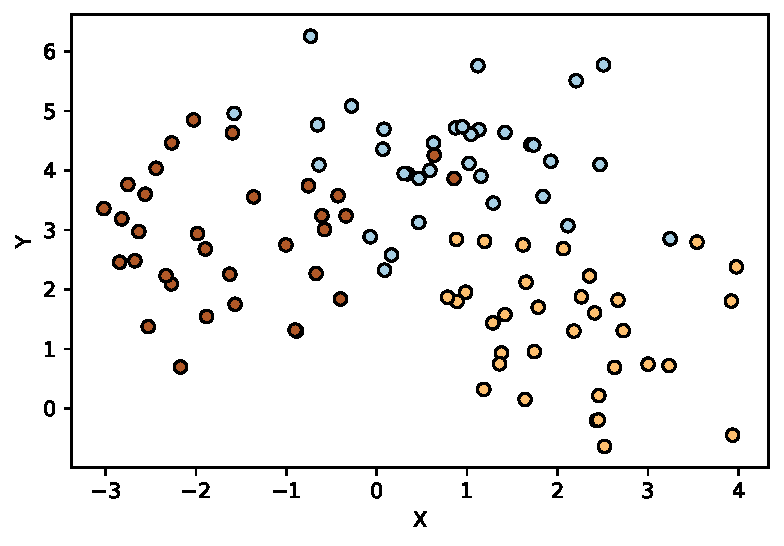
\includegraphics[width=0.6\linewidth]{knn/iris_knn_data.pdf}
    \caption{Randomly generated blobs}
\end{figure}
\end{frame}

\begin{frame}{Important Considerations: Distance Metric}
\only<1>{
\begin{columns}[T]
  \begin{column}{0.5\textwidth}
    \begin{figure}
      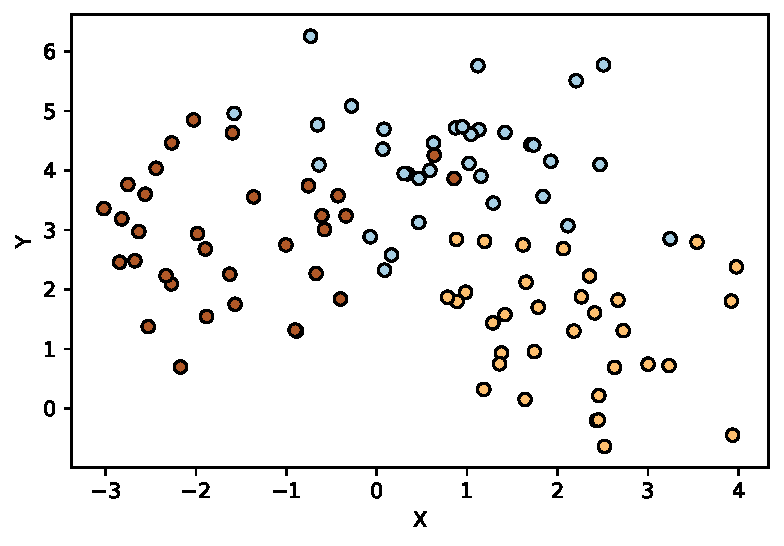
\includegraphics[width=\textwidth]{knn/iris_knn_data.pdf}
      %\vspace*{-0.3cm}
      \caption{Ground Truth}
    \end{figure}
  \end{column}
  \begin{column}{0.5\textwidth}
    \begin{figure}
      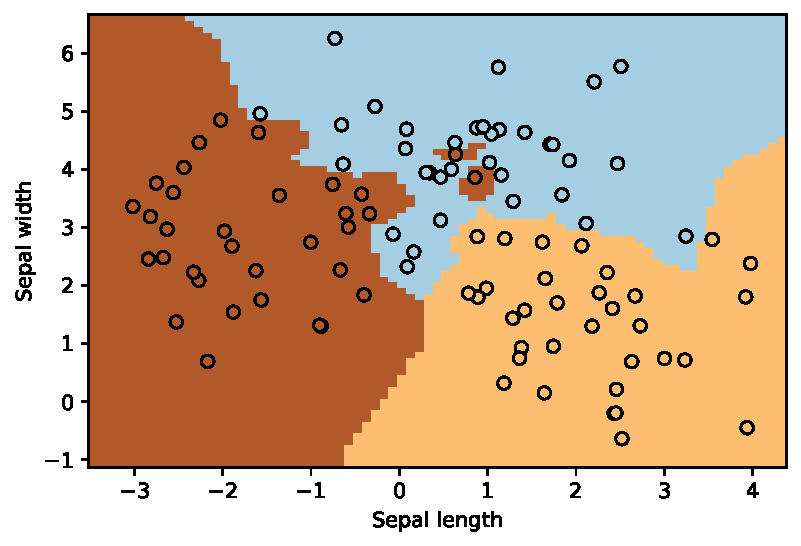
\includegraphics[width=\textwidth]{knn/iris_knn_def_1.pdf}
      %\vspace*{-0.3cm}
      \caption{Minskoaski = $\left(\sum|x-y|^p\right)^{\frac{1}{p}}$}
    \end{figure}
  \end{column}
\end{columns}}
\only<2>{
\begin{columns}[T]
  \begin{column}{0.5\textwidth}
    \begin{figure}
      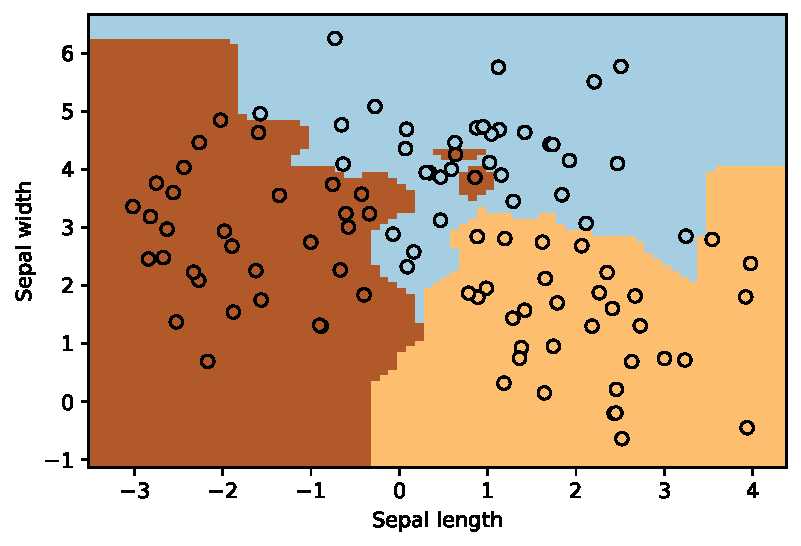
\includegraphics[width=\textwidth]{knn/iris_knn_man_1.pdf}
      %\vspace*{-0.3cm}
      \caption{Manhattan = $\sum|x-y|$}
    \end{figure}
  \end{column}
  \begin{column}{0.5\textwidth}
    \begin{figure}
      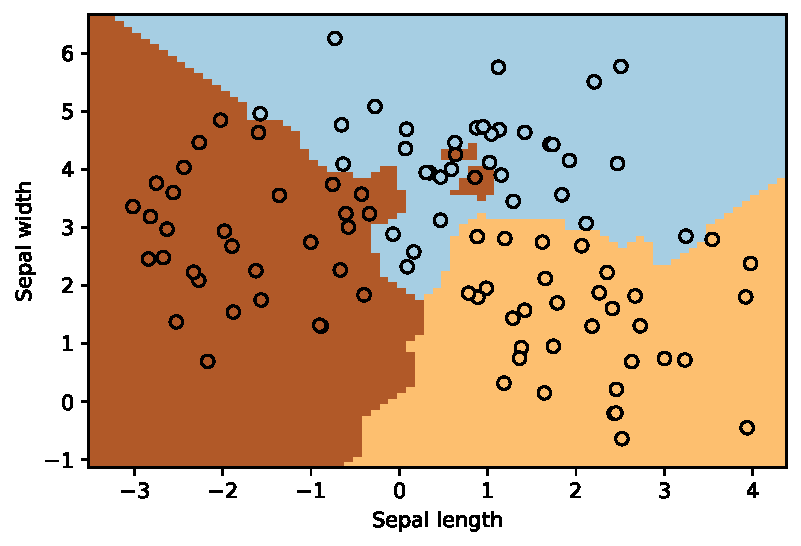
\includegraphics[width=\textwidth]{knn/iris_knn_che_1.pdf}
      %\vspace*{-0.3cm}
      \caption{Chebeshev = $\max|x-y|$}
    \end{figure}
  \end{column}
\end{columns}}
\end{frame}
\end{comment}
\begin{frame}{Important Considerations: Value of \emph{K}}
Choosing the correct value of \emph{K} is difficult.
\pause

\textbf{Low values of K} will result in each point having a very high influence on the final output $\implies$ noise will influence the result
\pause

\textbf{High values of K} will result in smoother decision boundaries \\$\implies$ lower variance but also higher bias
\end{frame}

\begin{frame}{Important Considerations: Value of \emph{K}}
\only<1>{\begin{columns}[T]
  \begin{column}{0.5\textwidth}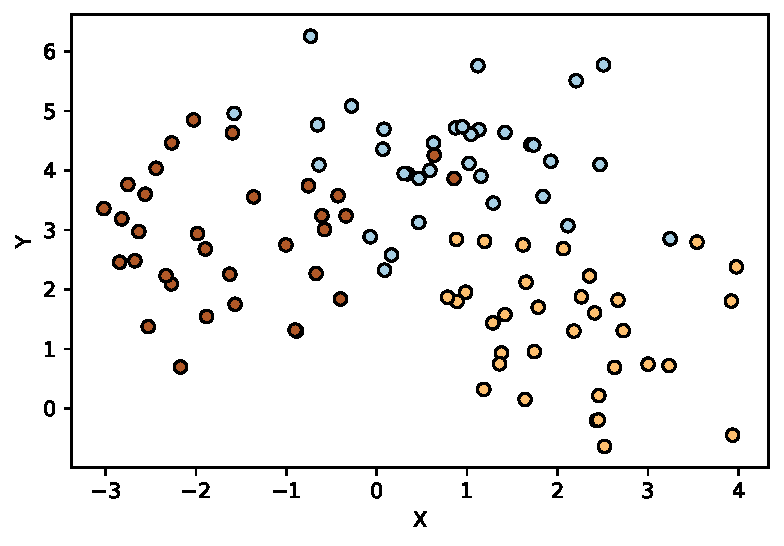
\includegraphics[height=0.7\textwidth]{knn/iris_knn_data.pdf}\captionof{figure}{Dataset}\end{column}
  \begin{column}{0.5\textwidth}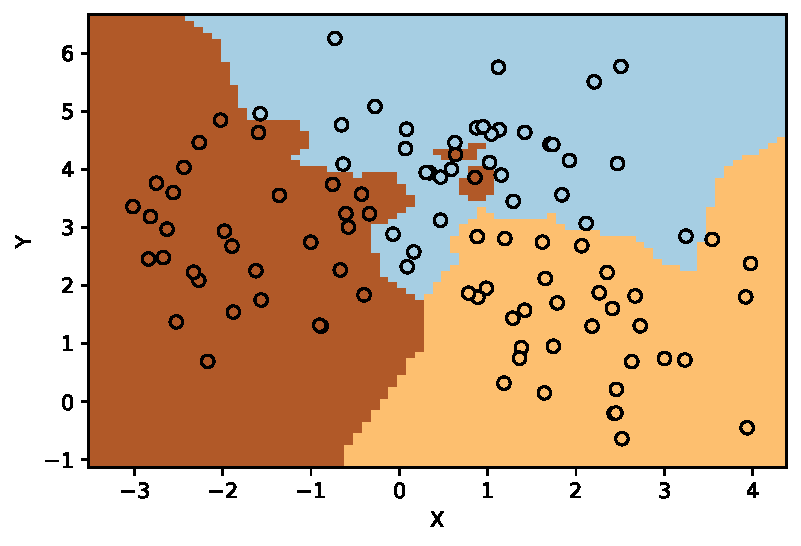
\includegraphics[height=0.7\textwidth]{knn/exp_knn_1.pdf}\captionof{figure}{K = 1 High Variance}\end{column}\end{columns}}
\only<2>{\begin{columns}[T]
  \begin{column}{0.5\textwidth}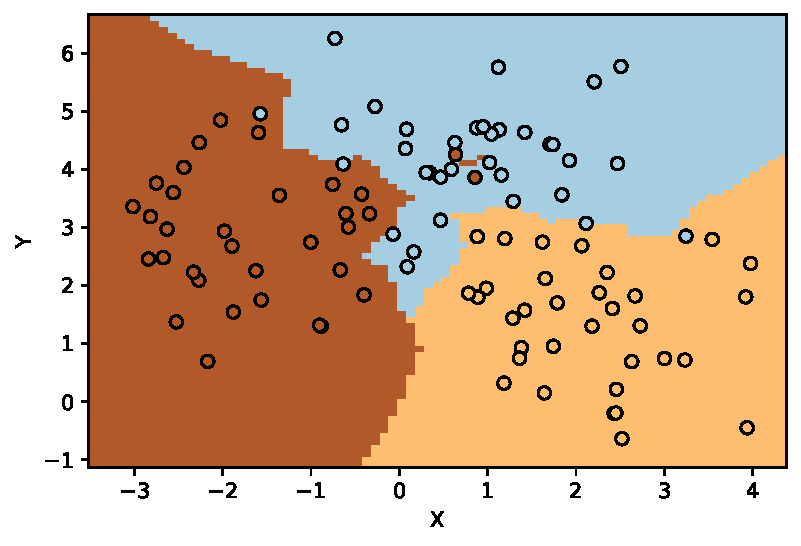
\includegraphics[height=0.7\textwidth]{knn/exp_knn_3.pdf}\captionof{figure}{K = 3}\end{column}
  \begin{column}{0.5\textwidth}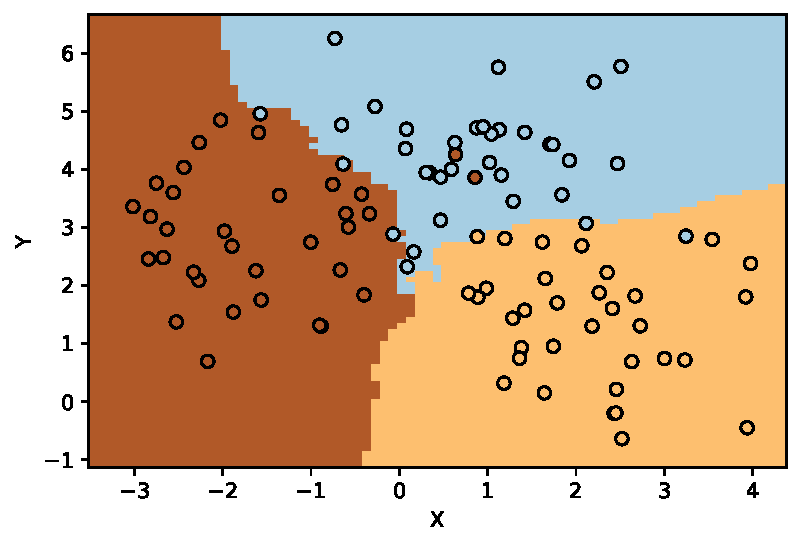
\includegraphics[height=0.7\textwidth]{knn/exp_knn_9.pdf}\captionof{figure}{K = 9 High Bias}\end{column}\end{columns}}

\end{frame}

%\begin{frame}{Important Considerations: Value of \emph{K}}
%\only<1>{\begin{columns}[T]
%  \begin{column}{0.5\textwidth}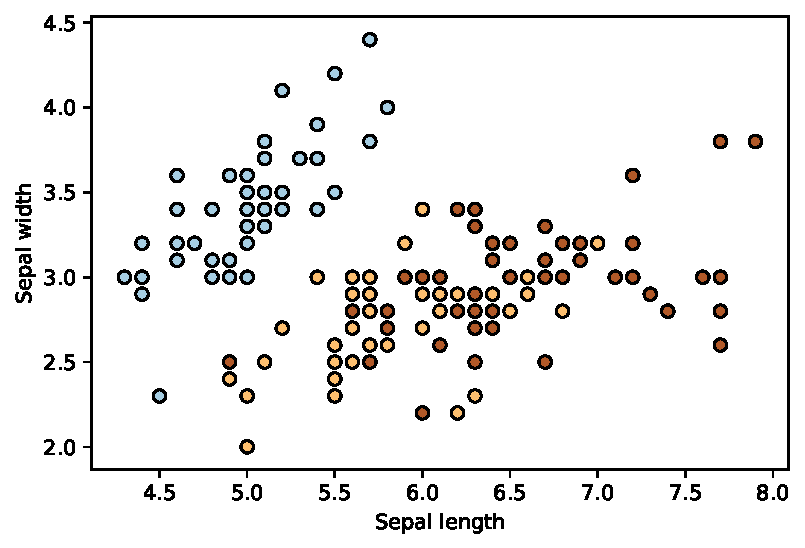
\includegraphics[height=0.7\textwidth]{knn/iris.pdf}\captionof{figure}{Iris Dataset}\end{column}
%  \begin{column}{0.5\textwidth}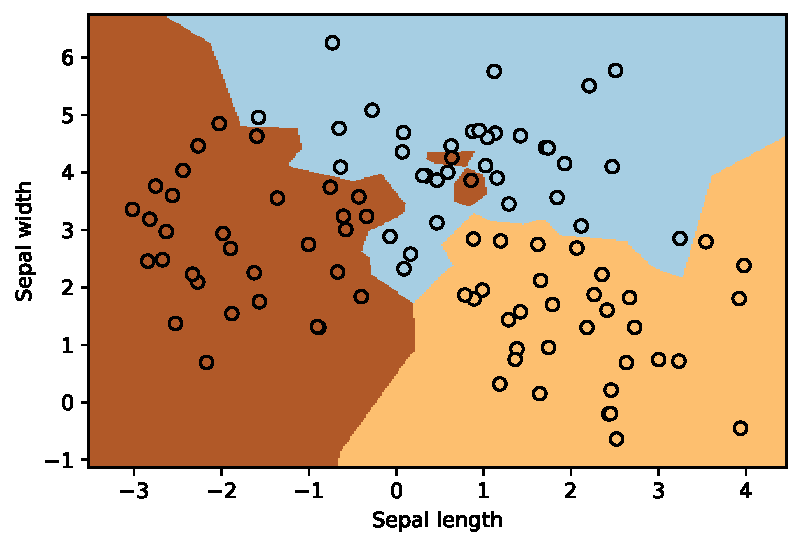
\includegraphics[height=0.7\textwidth]{knn/iris_knn_1.pdf}\captionof{figure}{K = 1}\end{column}\end{columns}}
%\only<2>{\begin{columns}[T]
%  \begin{column}{0.5\textwidth}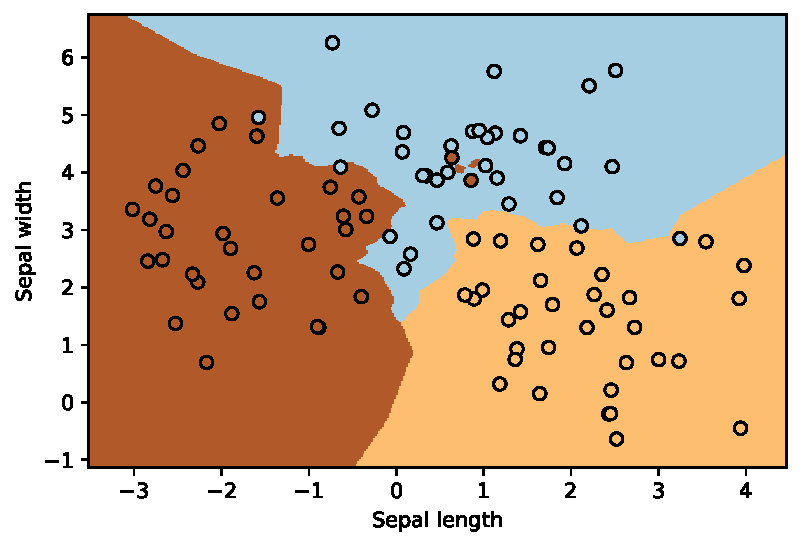
\includegraphics[height=0.7\textwidth]{knn/iris_knn_3.pdf}\captionof{figure}{K = 3}\end{column}
%  \begin{column}{0.5\textwidth}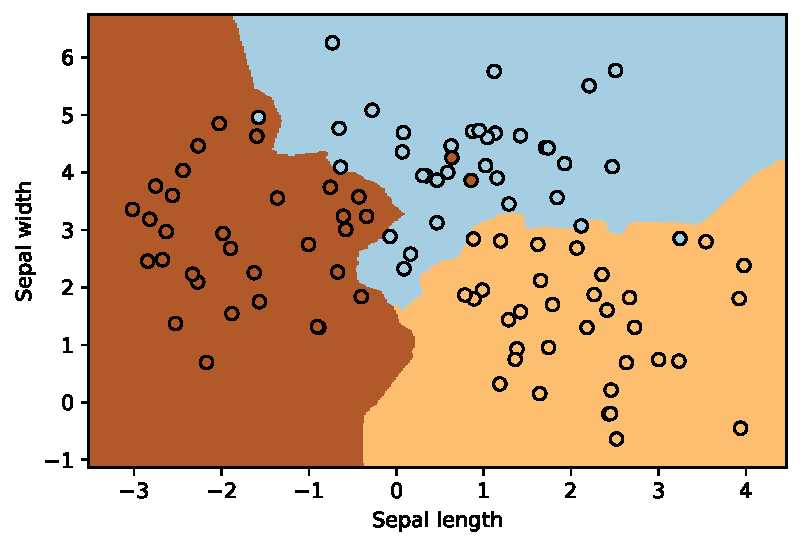
\includegraphics[height=0.7\textwidth]{knn/iris_knn_5.pdf}\captionof{figure}{K = 5}\end{column}\end{columns}}
%\only<3>{\begin{columns}[T]
%  \begin{column}{0.5\textwidth}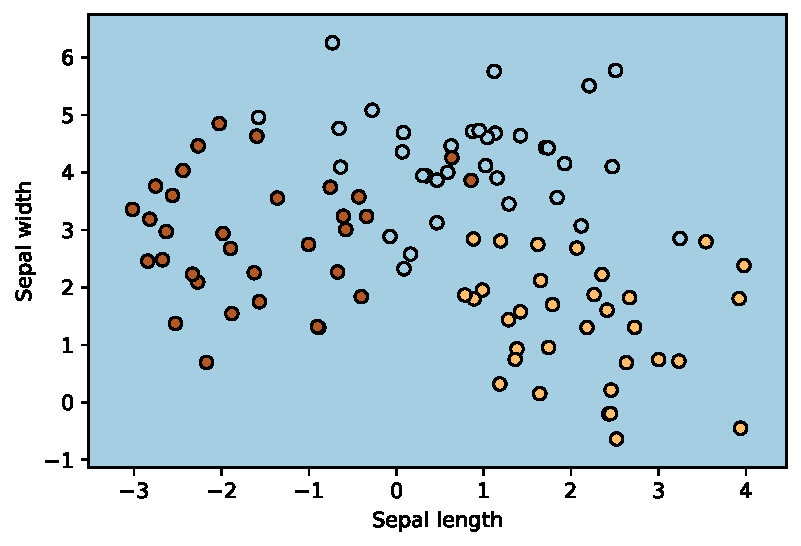
\includegraphics[height=0.7\textwidth]{knn/iris_knn_100.pdf}\captionof{figure}{K = 100}\end{column}
%  \begin{column}{0.5\textwidth}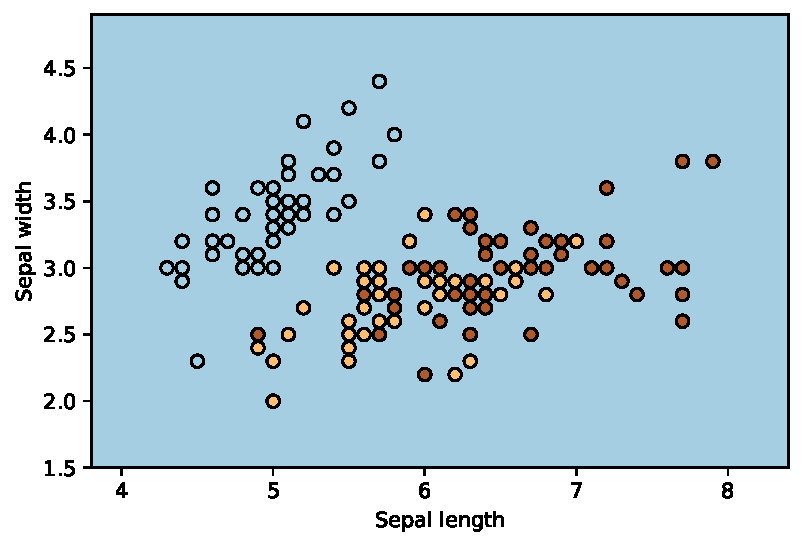
\includegraphics[height=0.7\textwidth]{knn/iris_knn_150.pdf}\captionof{figure}{K = 150}\end{column}\end{columns}}
%\end{frame}
\begin{comment}


\begin{frame}{Important Considerations: Aggregation Functions}
\only<1-2>{There are different ways to go about aggregating the data from the K nearest neighbors.}

\only<2>{\vspace{0.5cm} One method to do so would be to calculate the mean and choose the class that has the highest probability.}
\only<3>{\vspace{0.5cm}\begin{figure}
      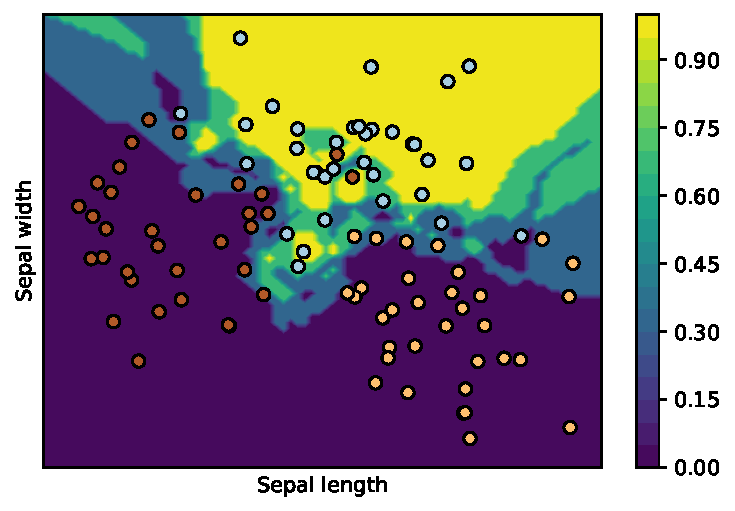
\includegraphics[width=0.8\textwidth]{knn/iris_prob_3_0.pdf}
      \caption{Probability Distribution for a point to belong to Class 0}
    \end{figure}
}

\only<4>{\vspace{0.5cm}\begin{columns}[T]
  \begin{column}{0.33\textwidth}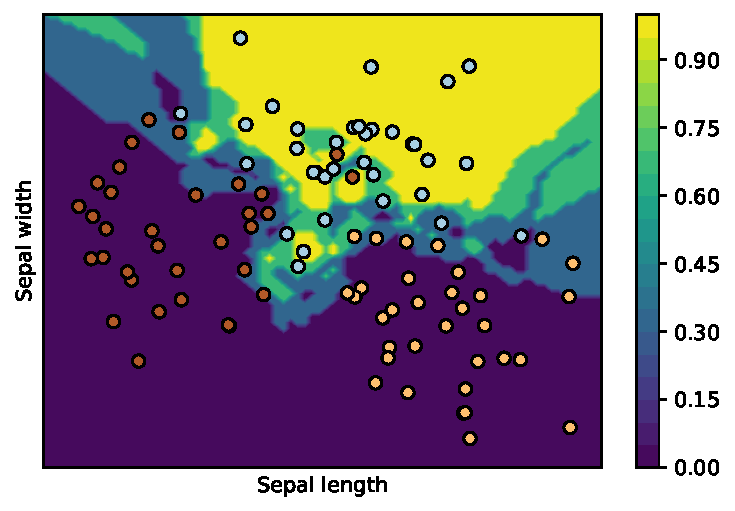
\includegraphics[height=0.7\textwidth]{knn/iris_prob_3_0.pdf}\captionof{figure}{K = 3 Class 1}\end{column}
  \begin{column}{0.33\textwidth}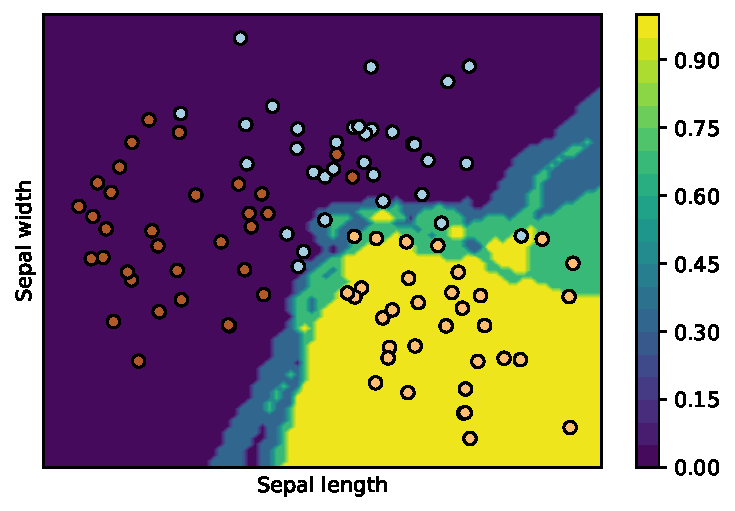
\includegraphics[height=0.7\textwidth]{knn/iris_prob_3_1.pdf}\captionof{figure}{K = 3 Class 2}\end{column}\begin{column}{0.33\textwidth}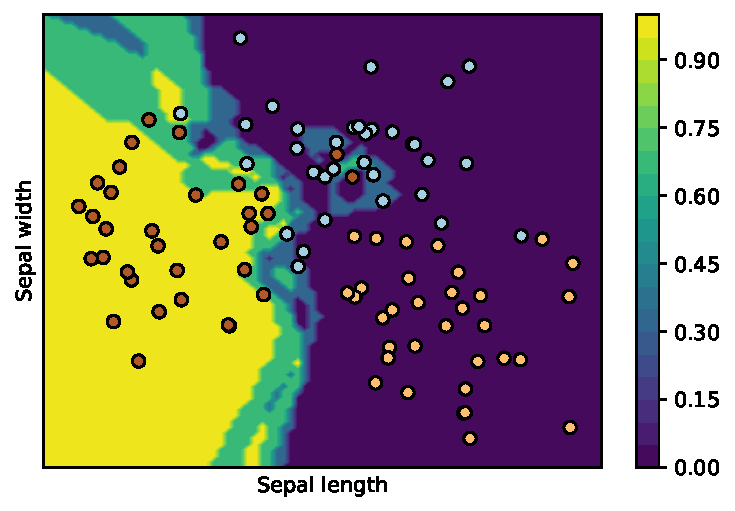
\includegraphics[height=0.7\textwidth]{knn/iris_prob_3_2.pdf}\captionof{figure}{K = 3 Class 3}\end{column}\end{columns}
  \vspace{1cm}
  \begin{columns}[T]
  \begin{column}{0.33\textwidth}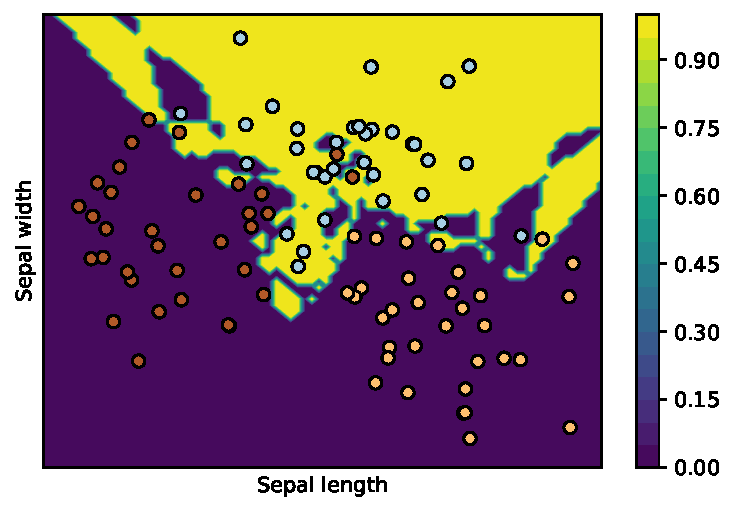
\includegraphics[height=0.7\textwidth]{knn/iris_prob_1_0.pdf}\captionof{figure}{K = 1 Class 1}\end{column}
  \begin{column}{0.33\textwidth}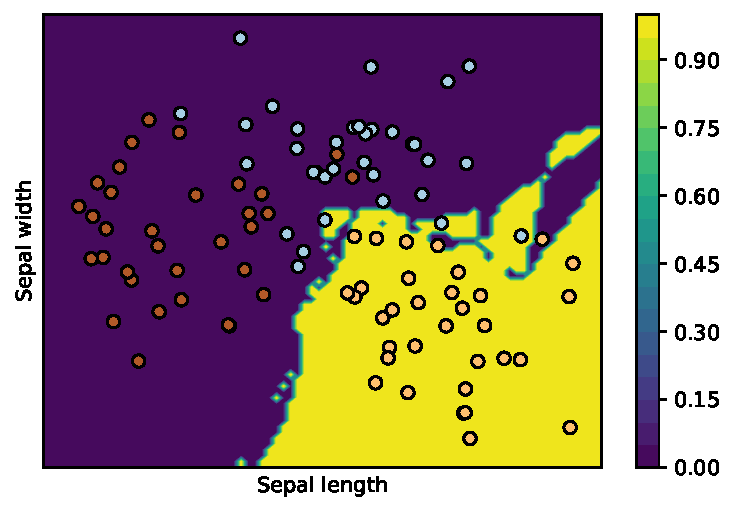
\includegraphics[height=0.7\textwidth]{knn/iris_prob_1_1.pdf}\captionof{figure}{K = 1 Class 2}\end{column}\begin{column}{0.33\textwidth}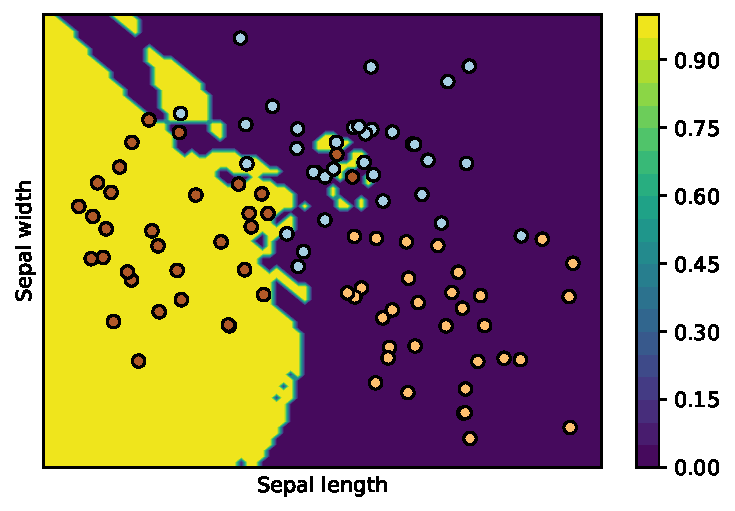
\includegraphics[height=0.7\textwidth]{knn/iris_prob_1_2.pdf}\captionof{figure}{K = 1 Class 3}\end{column}\end{columns}}
  
\only<5>{
There are different ways to go about aggregating the data from the K nearest neighbors.

\vspace{0.5cm} One method to do so would be to calculate the mean and choose the class that has the highest probability.

\vspace{0.5cm} Other methods include:
\begin{itemize}
\item Median
\item Mode
\end{itemize}
}
\end{frame}
\end{comment}

\begin{frame}{Aggregating data}
	There are different ways to go about aggregating the data from the K nearest neighbors.
	
	
	\begin{itemize}
		\item Median
		\item Mean
		\item Mode
	\end{itemize}
\end{frame}
\begin{frame}{KNN Algorithm}
\begin{itemize}
\item<1-> Keep the entire dataset: ${(x,y)}$
\item<2-> For a query vector $q$:
\begin{enumerate}
\item<3-> Find the k-closest data point(s) $x^*$
\item<4-> Predict $y^*$
\end{enumerate}
\end{itemize}
\end{frame}

\begin{frame}{Curse of Dimensionality}
With an increase in the number of dimensions:
\begin{enumerate}
\item<2-> the distance between points starts to increase
\item[]<2> {\centering 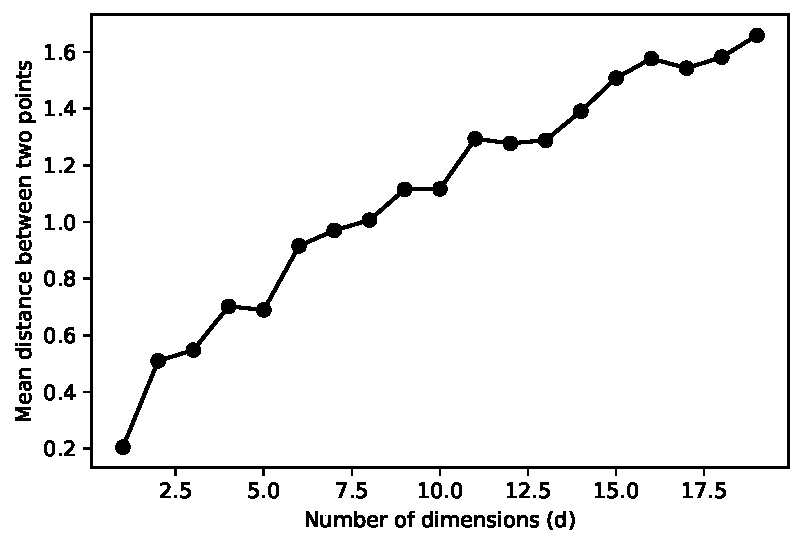
\includegraphics[height=0.6\textheight]{knn/curse_dist.pdf}}
\captionof{figure}{For a unifromly random dataset}
\end{enumerate}
\end{frame}

\begin{frame}{Curse of Dimensionality}
With an increase in the number of dimensions:
\begin{enumerate}
\item the distance between points starts to increase
\item the variation in distances between points starts to decrease
\item[] {\centering 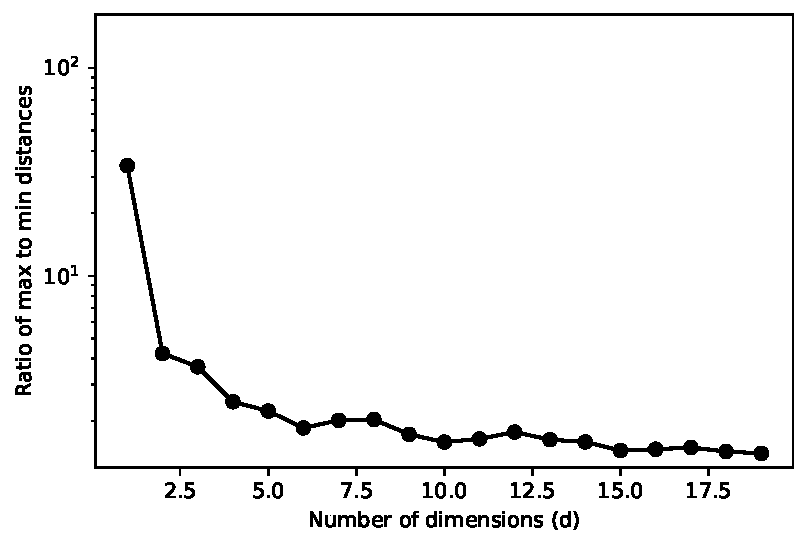
\includegraphics[height=0.6\textheight]{knn/curse_spread.pdf}}
\captionof{figure}{For a unifromly random dataset}
\end{enumerate}
\end{frame}

\begin{frame}{Curse of Dimensionality}
With an increase in the number of dimensions:
\begin{enumerate}
\item the distance between points starts to increase
\item the variation in distances between points starts to decrease
\end{enumerate}
Due to this, distance metrics lose their efficacy as a similarity metric.
\end{frame}

\begin{frame}{Approximate Nearest Neighbors}
\only<1>{\vspace{0.5cm}
Doing an exhaustive search over all the points is time consuming, especially if you have a large number of data points.
\begin{figure}
      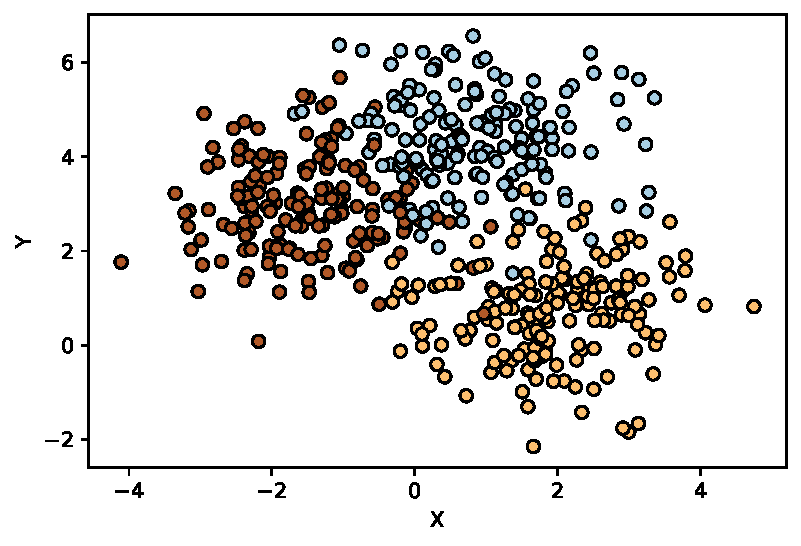
\includegraphics[width=0.6\textwidth]{knn/big.pdf}
      \caption{Example of a big dataset}
    \end{figure}}
\only<2->{
Doing an exhaustive search over all the points is time consuming, especially if you have a large number of data points.

If you are willing to sacrifice accuracy there are algorithms that can give you improvements that go into orders of magnitude.
}

\only<3->{
Such techniques include:
\begin{itemize}
\item<4-> Locality sensitive hashing
\item<5-> Vector approximation files
\item<6-> Greedy search in proximity neighborhood graphs
\end{itemize}
}
\end{frame}

\begin{frame}{Locality sensitive hashing}
\vspace{0.5cm}
\only<1-2>{Normal hash functions $H(x)$ try to keep the collision of points across bins uniform.}

\only<2->{A locality sensitive hash (LSH) function $L(x)$ would be designed such that similar values are mapped to similar bins. }

\only<3->{For such cases, all elements in a bin would be given the same label, which again can be decided on the basis of different aggregation methods}

\only<1->{
\begin{figure}
      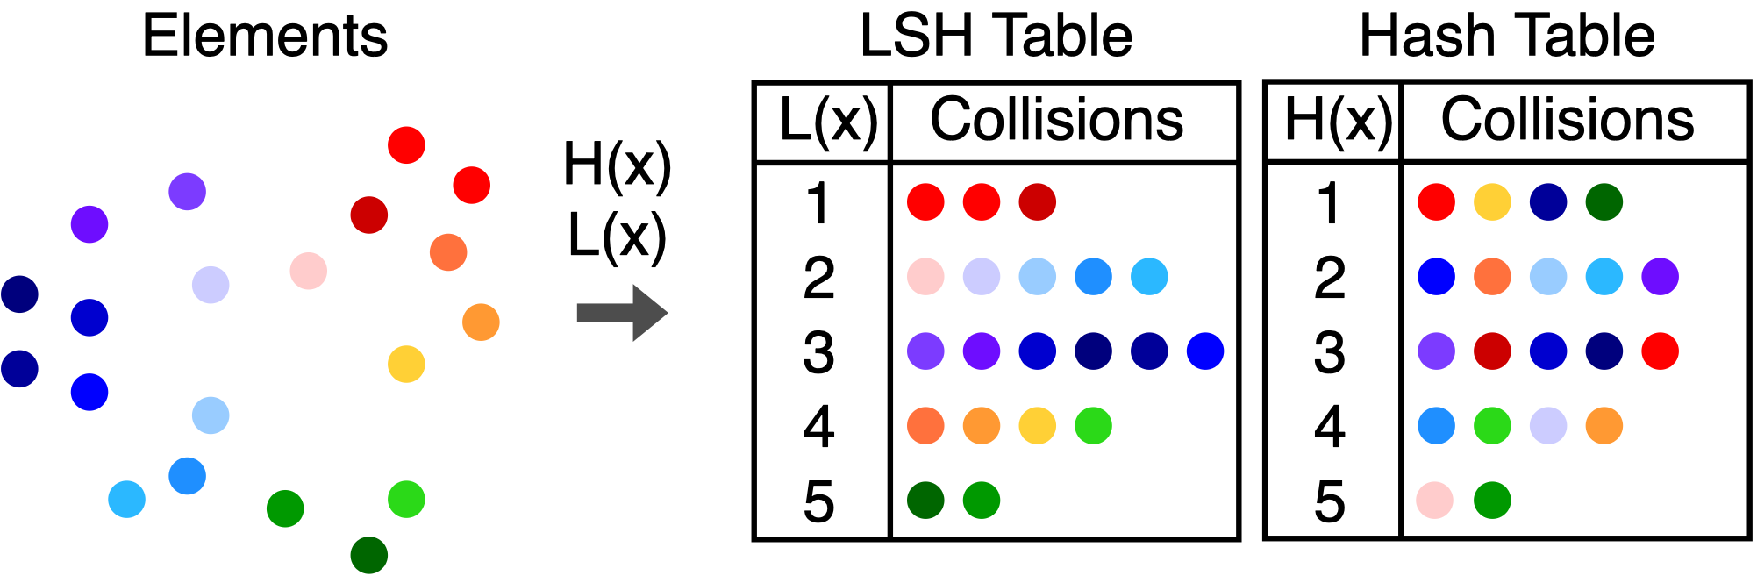
\includegraphics[width=0.8\textwidth]{knn/lsh.pdf}
      \caption{Example of a big dataset}
    \end{figure}}
\end{frame}
\end{document}
